% Copyright 2004 by Till Tantau <tantau@users.sourceforge.net>.
%
% In principle, this file can be redistributed and/or modified under
% the terms of the GNU Public License, version 2.
%
% However, this file is supposed to be a template to be modified
% for your own needs. For this reason, if you use this file as a
% template and not specifically distribute it as part of a another
% package/program, I grant the extra permission to freely copy and
% modify this file as you see fit and even to delete this copyright
% notice. 

\documentclass{beamer}
\usepackage{caption}
\usepackage{subcaption}
\usepackage{wrapfig}
\usepackage{animate}
\usepackage{natbib}
% There are many different themes available for Beamer. A comprehensive
% list with examples is given here:
% http://deic.uab.es/~iblanes/beamer_gallery/index_by_theme.html
% You can uncomment the themes below if you would like to use a different
% one:
%\usetheme{AnnArbor}
%\usetheme{Antibes}
%\usetheme{Bergen}
%\usetheme{Berkeley}
%\usetheme{Berlin}
%\usetheme{Boadilla}
%\usetheme{boxes}
%\usetheme{CambridgeUS}
%\usetheme{Copenhagen}
%\usetheme{Darmstadt}
%\usetheme{default}
%\usetheme{Frankfurt}
\usetheme{Goettingen}
%\usetheme{Hannover}      % the best till now, USE THIS
%\usetheme{Ilmenau}
%\usetheme{JuanLesPins}
%\usetheme{Luebeck}
%\usetheme{Madrid}        %was using this
%\usetheme{Malmoe}
%\usetheme{Marburg}
%\usetheme{Montpellier}
%\usetheme{PaloAlto}
%\usetheme{Pittsburgh}
%\usetheme{Rochester}
%\usetheme{Singapore}    % pretty good, has a progress bar on top
%\usetheme{Szeged}
%\usetheme{Warsaw}

\setbeamertemplate{caption}[numbered]
%\DeclareCaptionFont{xxviii}{\fontsize{8}{10}\selectfont}
%\captionsetup{font=xxviii}
%\subcaptionsetup{font=xxviii}


\title{Climate: A whirlwind tour}

% A subtitle is optional and this may be deleted
\subtitle{\small Open Seminar Series, Department of Physics}

\author{Aditya Narayanan \thanks{adityarn@gmail.com, https://github.com/adityarn/presentations}}
% - Give the names in the same order as the appear in the paper.
% - Use the \inst{?} command only if the authors have different
%   affiliation.

\institute[IITM] % (optional, but mostly needed)
{
  Department of Ocean Engineering\\
  IIT Madras}
% - Use the \inst command only if there are several affiliations.
% - Keep it simple, no one is interested in your street address.

\date{October, 2018}
% - Either use conference name or its abbreviation.
% - Not really informative to the audience, more for people (including
%   yourself) who are reading the slides online

\subject{Climate Science}
% This is only inserted into the PDF information catalog. Can be left
% out. 

% If you have a file called "university-logo-filename.xxx", where xxx
% is a graphic format that can be processed by latex or pdflatex,
% resp., then you can add a logo as follows:

% \pgfdeclareimage[height=0.5cm]{university-logo}{university-logo-filename}
% \logo{\pgfuseimage{university-logo}}

% Delete this, if you do not want the table of contents to pop up at
% the beginning of each subsection:
%% \AtBeginSubsection[]
%% {
%%   \begin{frame}<beamer>{Outline}
%%     \tableofcontents[currentsection,currentsubsection]
%%   \end{frame}
%% }

% Let's get started
\begin{document}

\begin{frame}
  \titlepage
\end{frame}

%% \begin{frame}{Outline}
%%   \tableofcontents
%%   % You might wish to add the option [pausesections]
%% \end{frame}

% Section and subsections will appear in the presentation overview
% and table of contents.
\section{Introduction and motivation}

\begin{frame}{Climate change}
\begin{figure}
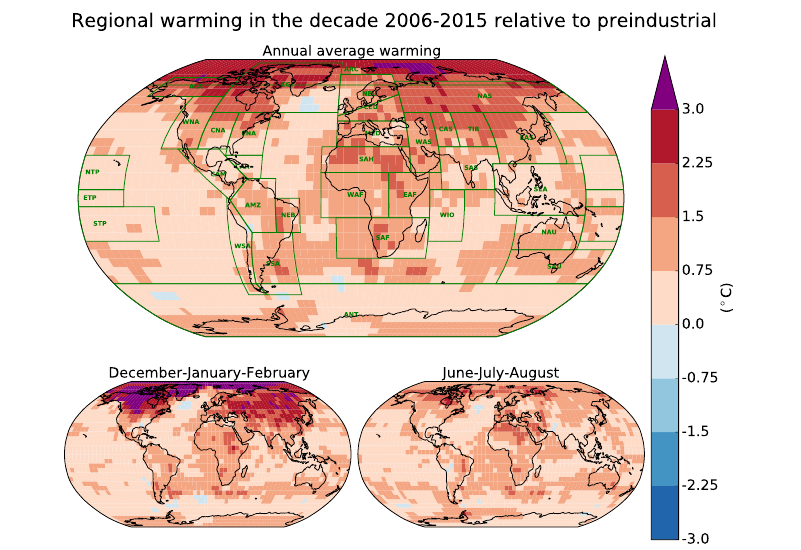
\includegraphics[width=\linewidth]{./Images/RegionalWarming_2006_2015}
\caption{\label{fig:RegWarming} Temperature change (2005 - 2015) with respect to pre-industrial (1850-1900). {\tiny Source: \href{http://www.ipcc.ch/report/sr15/}{\textit{IPCC SR15, 2018.}}}}
\end{figure}
\end{frame}

\begin{frame}{Historical CO$_2$ levels}
\begin{figure}
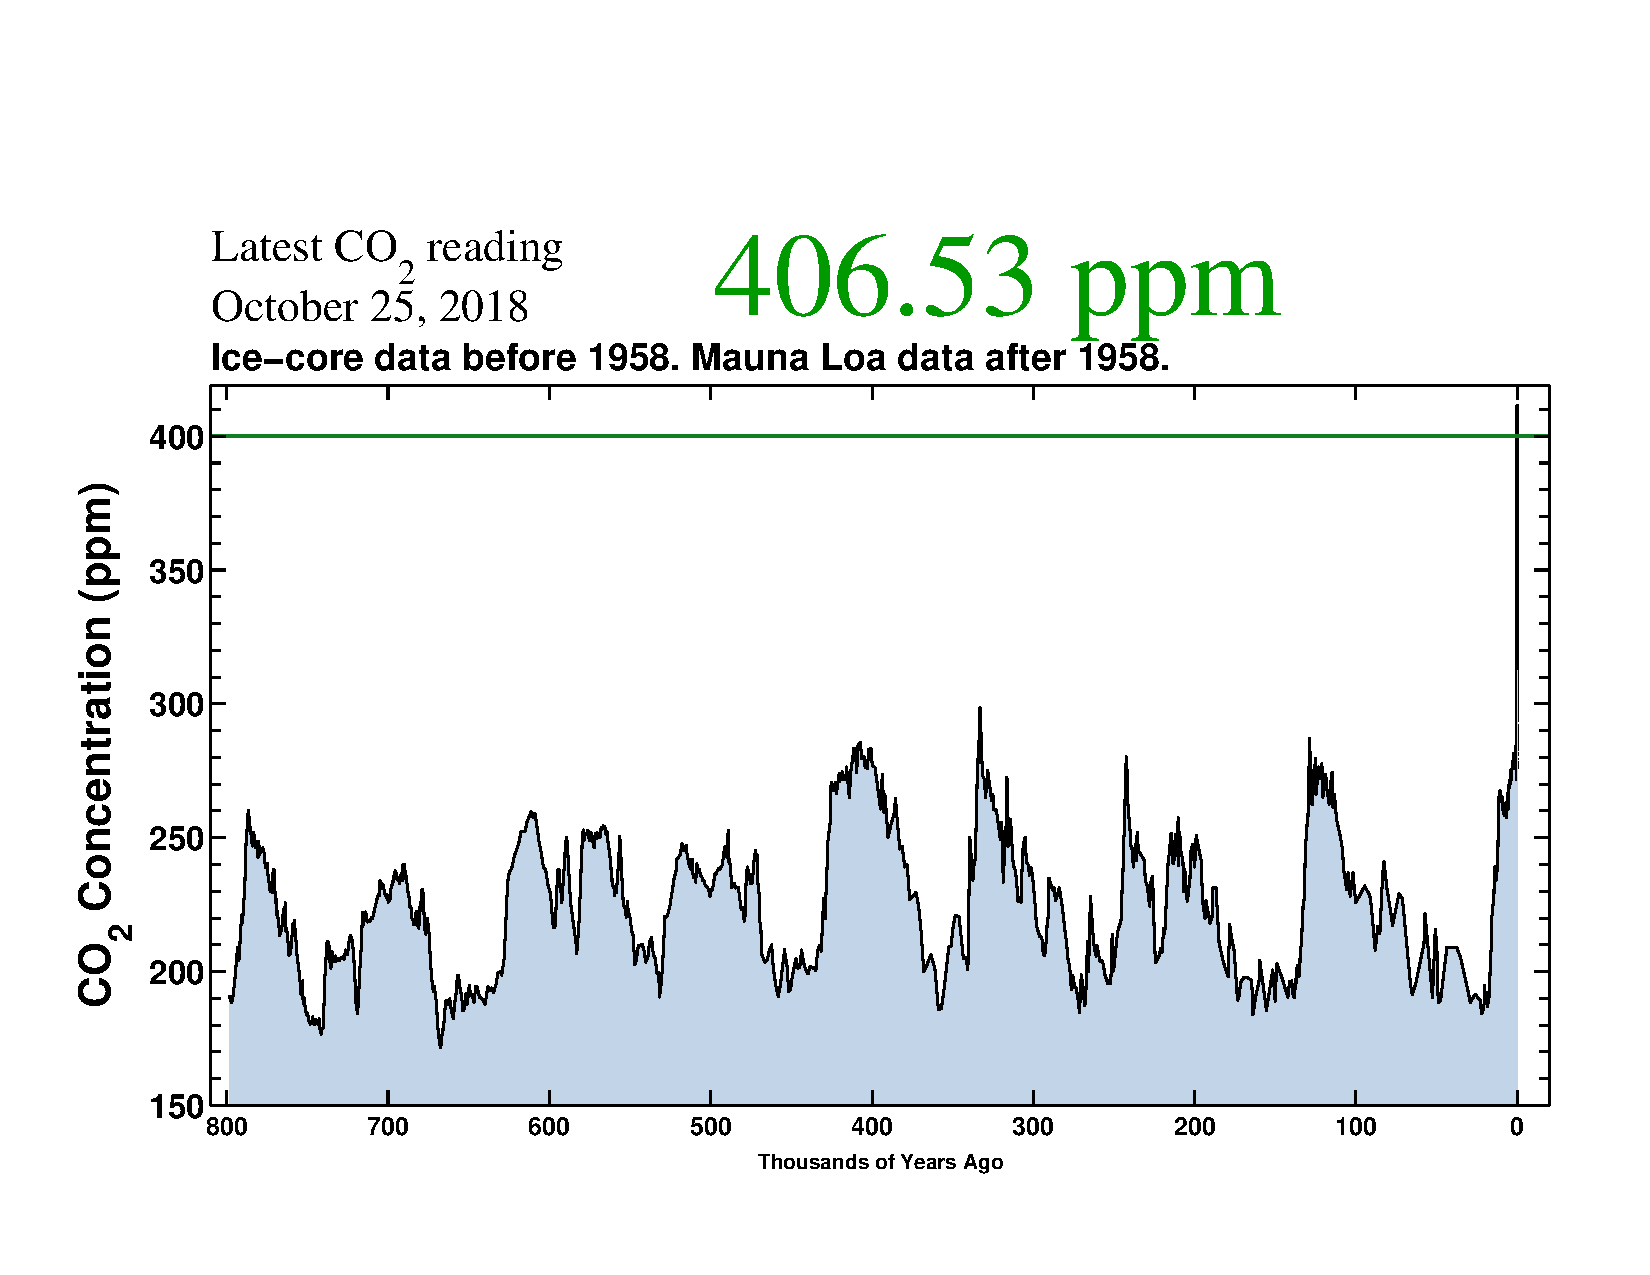
\includegraphics[width=\linewidth]{./Images/co2_800k}
\caption{\label{fig:CO2} Historical CO$_2$ levels. {\tiny Source: \href{https://scripps.ucsd.edu/programs/keelingclone/wp-content/plugins/sio-bluemoon/graphs/co2_800k.pdf}{\textit{Scripps, UCSD}}}}
\end{figure}
\end{frame}

\begin{frame}{Palaeo record}
\begin{figure}
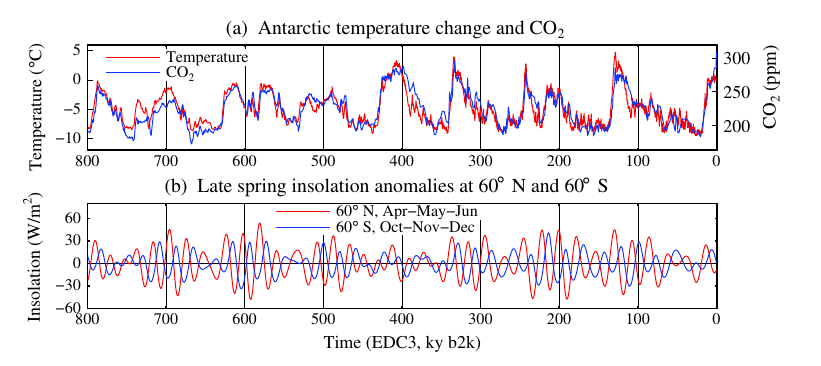
\includegraphics[width=\linewidth]{./Images/PaleoTemp_CO2_Insolation.png}
\caption{\label{fig:Palaeo} ({\bf a}) Antarctic (Dome C) temperature anomaly relative to 10kya, CO$_2$ levels \citep{luthi2008PalaeoCO2}; ({\bf b}) Insolation anomalies. {\tiny Source: \citep{hansen2016IceMelt}}}
\end{figure}
\end{frame}


\begin{frame}{Radiative forcing}
\begin{figure}
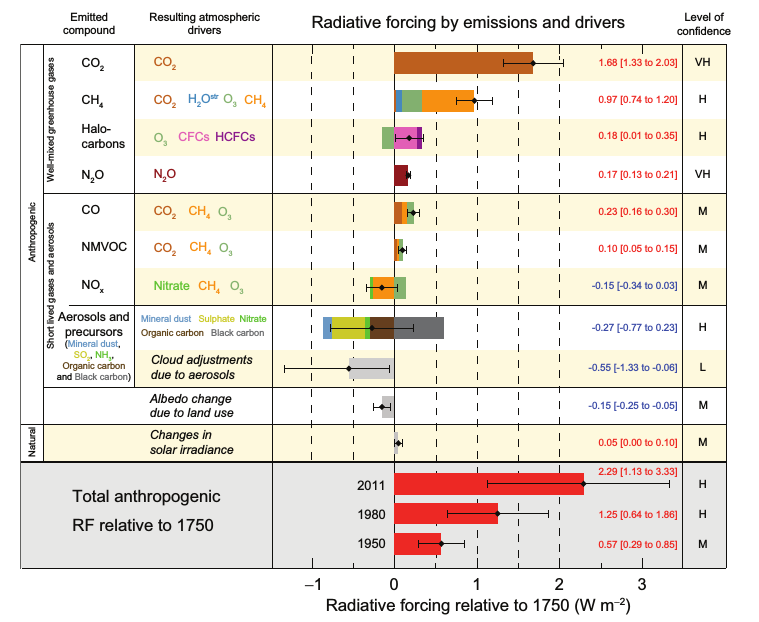
\includegraphics[width=0.9\linewidth]{./Images/radiativeForcing_IPCC2013.png}
\caption{\label{fig:RF} Radiative forcing. \href{http://www.ipcc.ch/report/ar5/wg1/}{\tiny Source: IPCC-WG1, 2013}}
\end{figure}
\end{frame}


\section{Atmosphere}

\begin{frame}{Earth's energy budget}
\begin{figure}
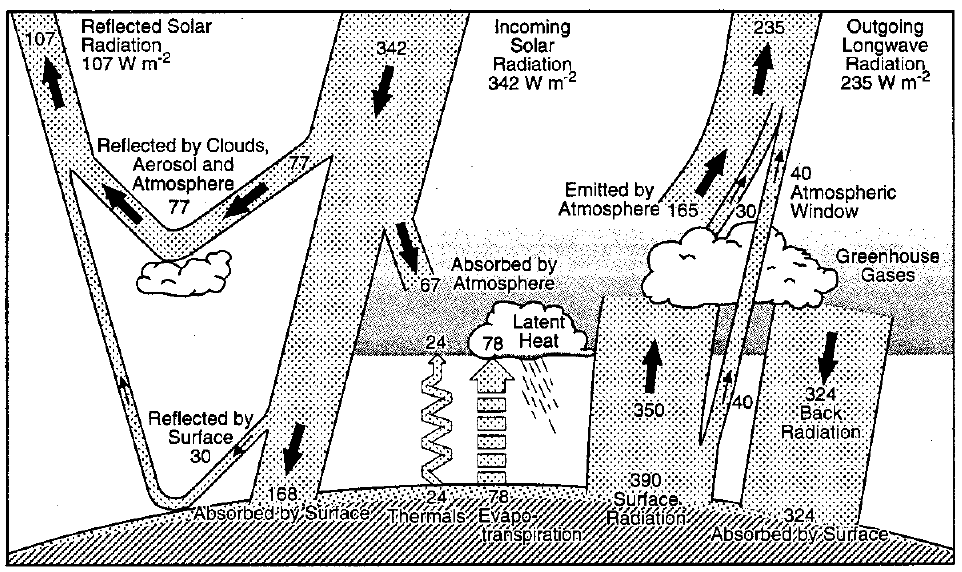
\includegraphics[width=\linewidth]{./Images/Trenberth2013_EnergyBudget.png}
\caption{\label{fig:EnergyBudget} \href{https://journals.ametsoc.org/doi/abs/10.1175/1520-0477(1997)078\%3C0197:EAGMEB\%3E2.0.CO;2}{\tiny \citep{kiehl1997EnergyBudget} } }
\end{figure}
\end{frame}

\begin{frame}{Aerosols}
\begin{figure}
\includegraphics[width=\linewidth]{./Images/AerosolEarth_NASA.jpg}
\caption{\label{fig:Aerosols} Wildfires, dust, and sea salt - August 23rd, 2018. \href{https://earthobservatory.nasa.gov/images/92654/just-another-day-on-aerosol-earth}{\tiny Source: NASA GEOS-FP } }
\end{figure}
\end{frame}



\section{Biosphere}

\begin{frame}
\begin{figure}
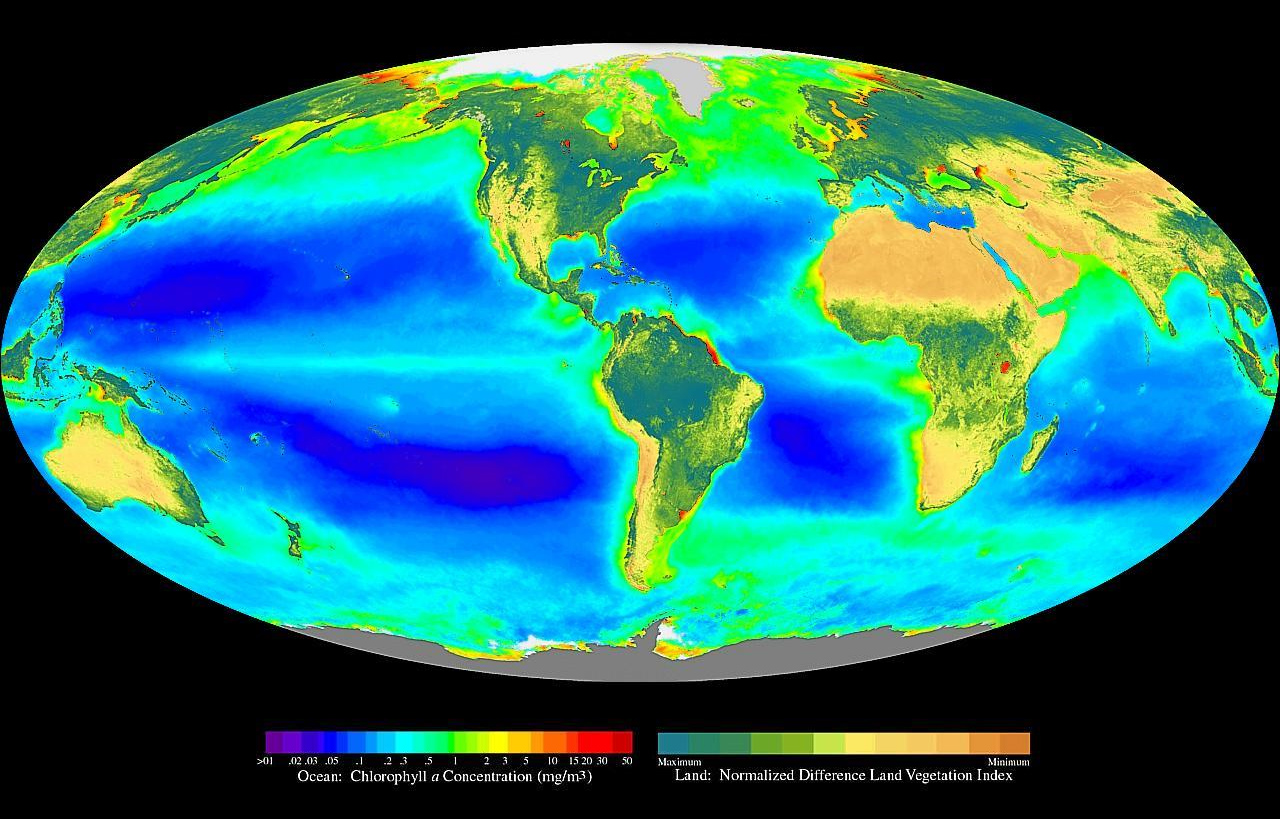
\includegraphics[width=0.9\linewidth]{./Images/Seawifs_global_biosphere.jpg}
\caption{\label{fig:NPP} Abundance of photosynthesizing organisms. \href{http://oceancolor.gsfc.nasa.gov/SeaWiFS/BACKGROUND/Gallery/index.html}{\tiny Source: NASA, GSFC (SeaWiFS)}}
\end{figure}
\end{frame}


\begin{frame}{Biophysical feedbacks}
\begin{figure}
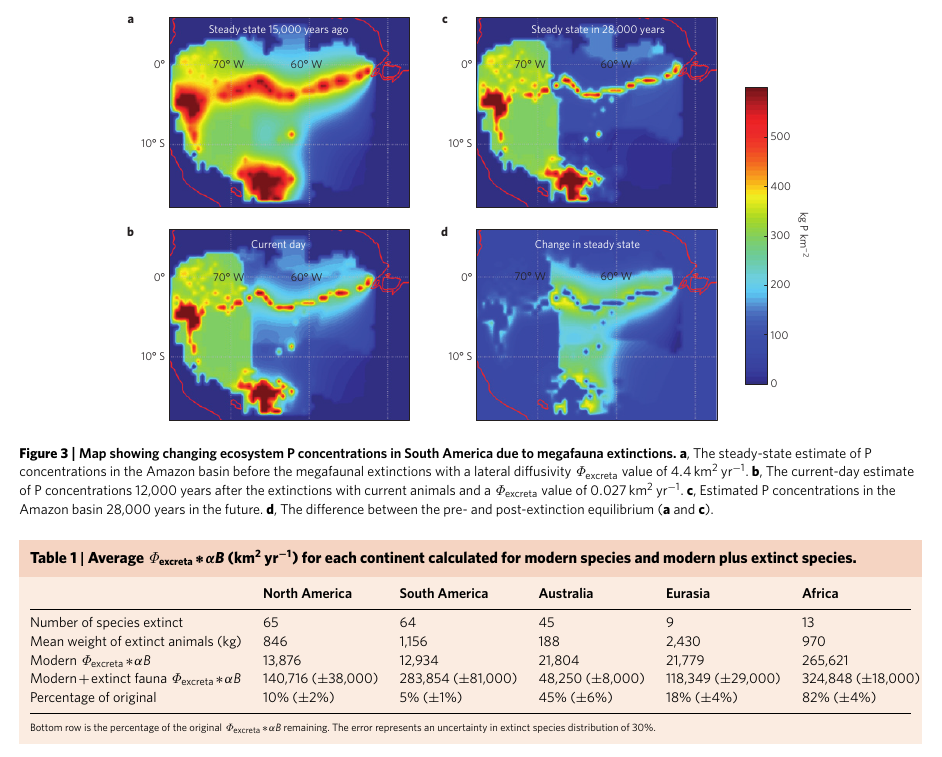
\includegraphics[width=\linewidth]{./Images/AmazonNutrient_doughty2013.png}
\caption{\label{fig:AmazonP} \href{https://www.nature.com/articles/ngeo1895}{\tiny Source: \citep{doughty2013AmazonNutrient} }}
\end{figure}
\end{frame}


\begin{frame}
\begin{figure}
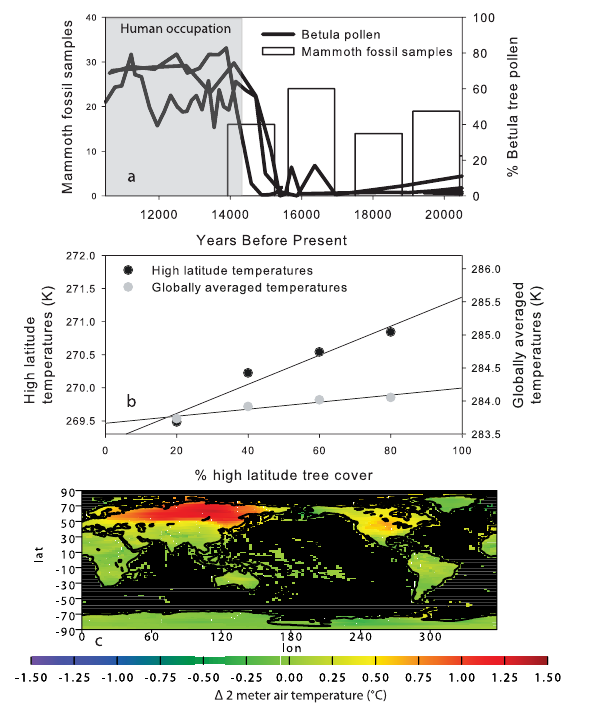
\includegraphics[width=0.7\linewidth]{./Images/doughty_betula_2010.png}
\caption{\label{fig:Betula} \href{https://agupubs.onlinelibrary.wiley.com/doi/full/10.1029/2010GL043985}{\tiny Source: \citep{doughty2010Betula} }}
\end{figure}
\end{frame}



\begin{frame}
\begin{figure}
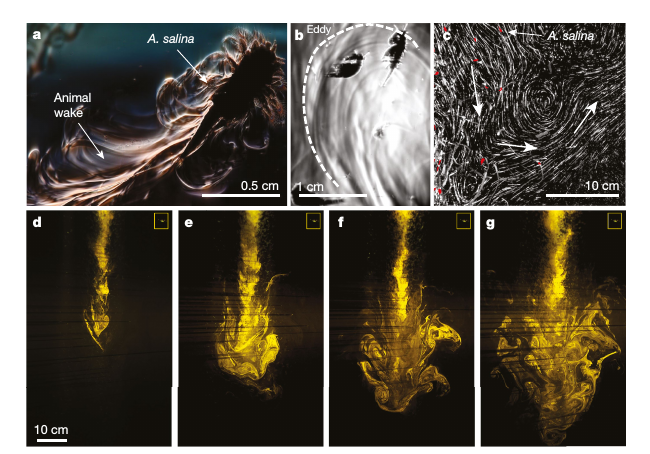
\includegraphics[width=\linewidth]{./Images/Swimmer_Visualization.png}
\caption{\label{fig:SwimmerDiffusion} Flow visualization of diffusion caused by the vertical migration of A. Salina (brine shrimp). $\nu_{eff} / \nu_{mol} \approx 10^3$ \href{https://www.nature.com/articles/s41586-018-0044-z}{\tiny Source: \citep{houghton2018SwimmerDiffusion} }}
\end{figure}
\end{frame}



\section{Ocean and the cryosphere}

\begin{frame}{Thermohaline circulation}
\begin{figure}
\captionsetup[figure]{font=scriptsize,labelfont=scriptsize}
\captionsetup[subfigure]{font=scriptsize,labelfont=scriptsize}
\centering
\includegraphics[width=0.9\linewidth]{/media/work/Literature/Charts_Maps/My_illustrations/LumpkinSpeer2007_thermohaline.png}
\caption{\label{fig:LumpkinSpeer2007} Global thermohaline circulation {\tiny source: Lumpkin and Speer, 2007 \citep{lumpkin2007global}}}
\end{figure}
\end{frame}


\begin{frame}
\begin{figure}
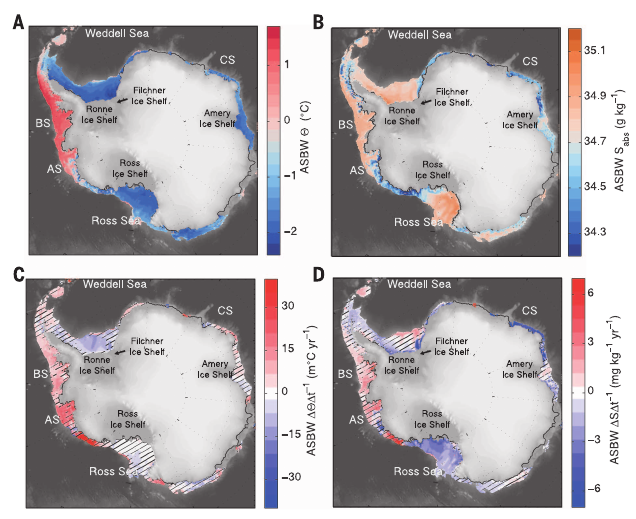
\includegraphics[width=\linewidth]{./Images/Schmidtko_ASBW_2014.png}
\caption{\label{fig:SchmidtkoASBW} Antarctic shelf sea bottom water properties and trends. \href{http://science.sciencemag.org/content/346/6214/1227}{\tiny Source: \citep{schmidtko2014multidecadal} }}
\end{figure}
\end{frame}


\begin{frame}
\begin{figure}
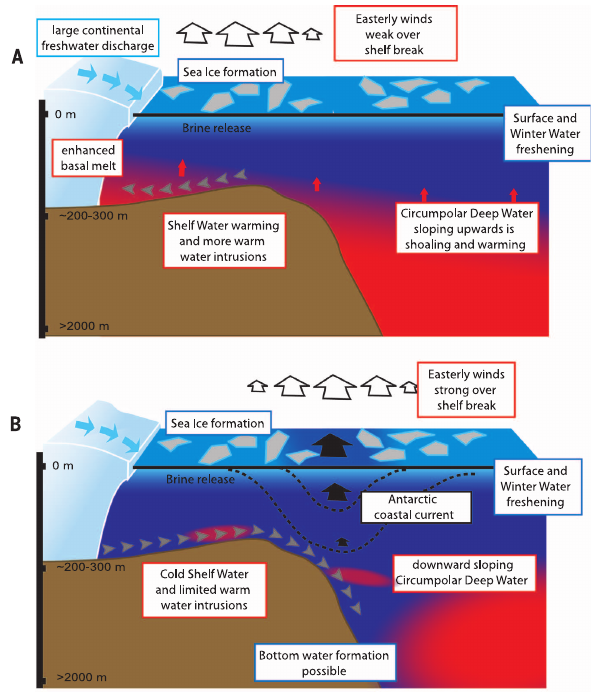
\includegraphics[width=0.7\linewidth]{./Images/SchmidtkoIllustration_2014.png}
\caption{\label{fig:SchmidtkoIllustration} Mechanisms of ocean currents warming the continental ice shelves of the Antarctic. \href{http://science.sciencemag.org/content/346/6214/1227}{\tiny Source: \citep{schmidtko2014multidecadal} }}
\end{figure}
\end{frame}


\begin{frame}
\begin{figure}
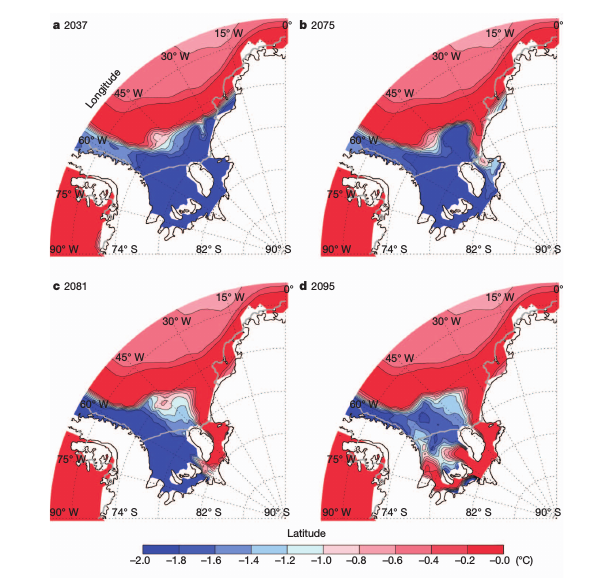
\includegraphics[width=0.7\linewidth]{./Images/Hellmer2012_CDWshoaling.png}
\caption{\label{fig:HellmerCDW} Modelling the future shelf bed of the Weddell Sea. \href{https://www.nature.com/articles/nature11064}{\tiny Source: \citep{hellmer2012} }}
\end{figure}
\end{frame}



\begin{frame}
\begin{figure}
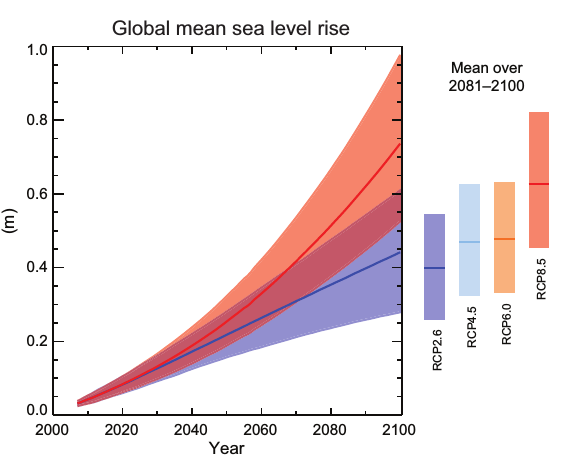
\includegraphics[width=\linewidth]{./Images/IPCC_GMSL_2100.png}
\caption{\label{fig:IPCC_SLR} IPCC 2013, sea level rise projections. \href{http://www.ipcc.ch/report/ar5/}{\tiny Source: IPCC 2013, AR5-WG1 }}
\end{figure}
\end{frame}


\begin{frame}
\begin{figure}
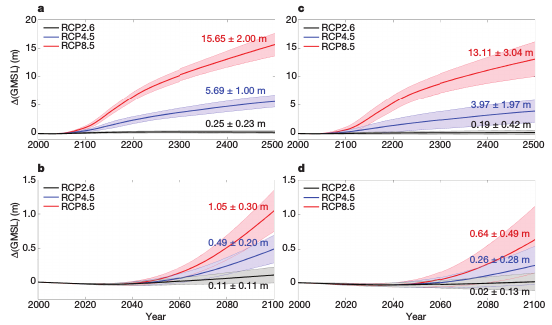
\includegraphics[width=\linewidth]{./Images/Deconto_2016_SLR.png}
\caption{\label{fig:DeContoSLR} Model analyses of future Antarctic contribution to sea level rise. \href{https://www.nature.com/articles/nature17145}{\tiny Source: \citep{deconto2016AntSLR} }}
\end{figure}
\end{frame}



\section{Mitigation and policy}

\begin{frame}
\begin{figure}
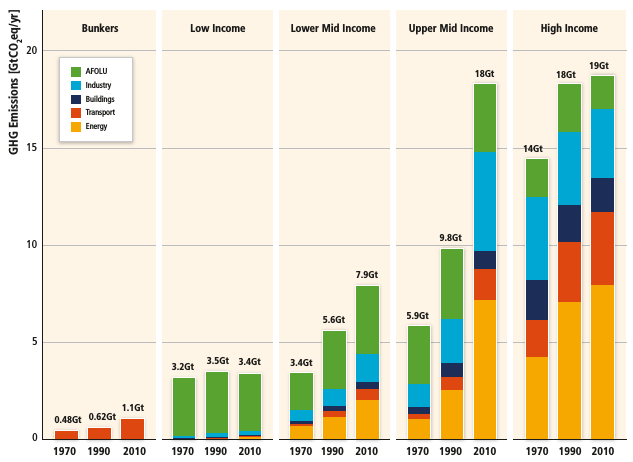
\includegraphics[width=\linewidth]{./Images/Emissions_byIncome.png}
\caption{\label{fig:EmissionsIncome} \href{http://www.ipcc.ch/pdf/assessment-report/ar5/wg3/ipcc_wg3_ar5_full.pdf}{\tiny Source: Fig. TS3, IPCC, 2013, WG-3 }}
\end{figure}
\end{frame}

\begin{frame}
\begin{figure}
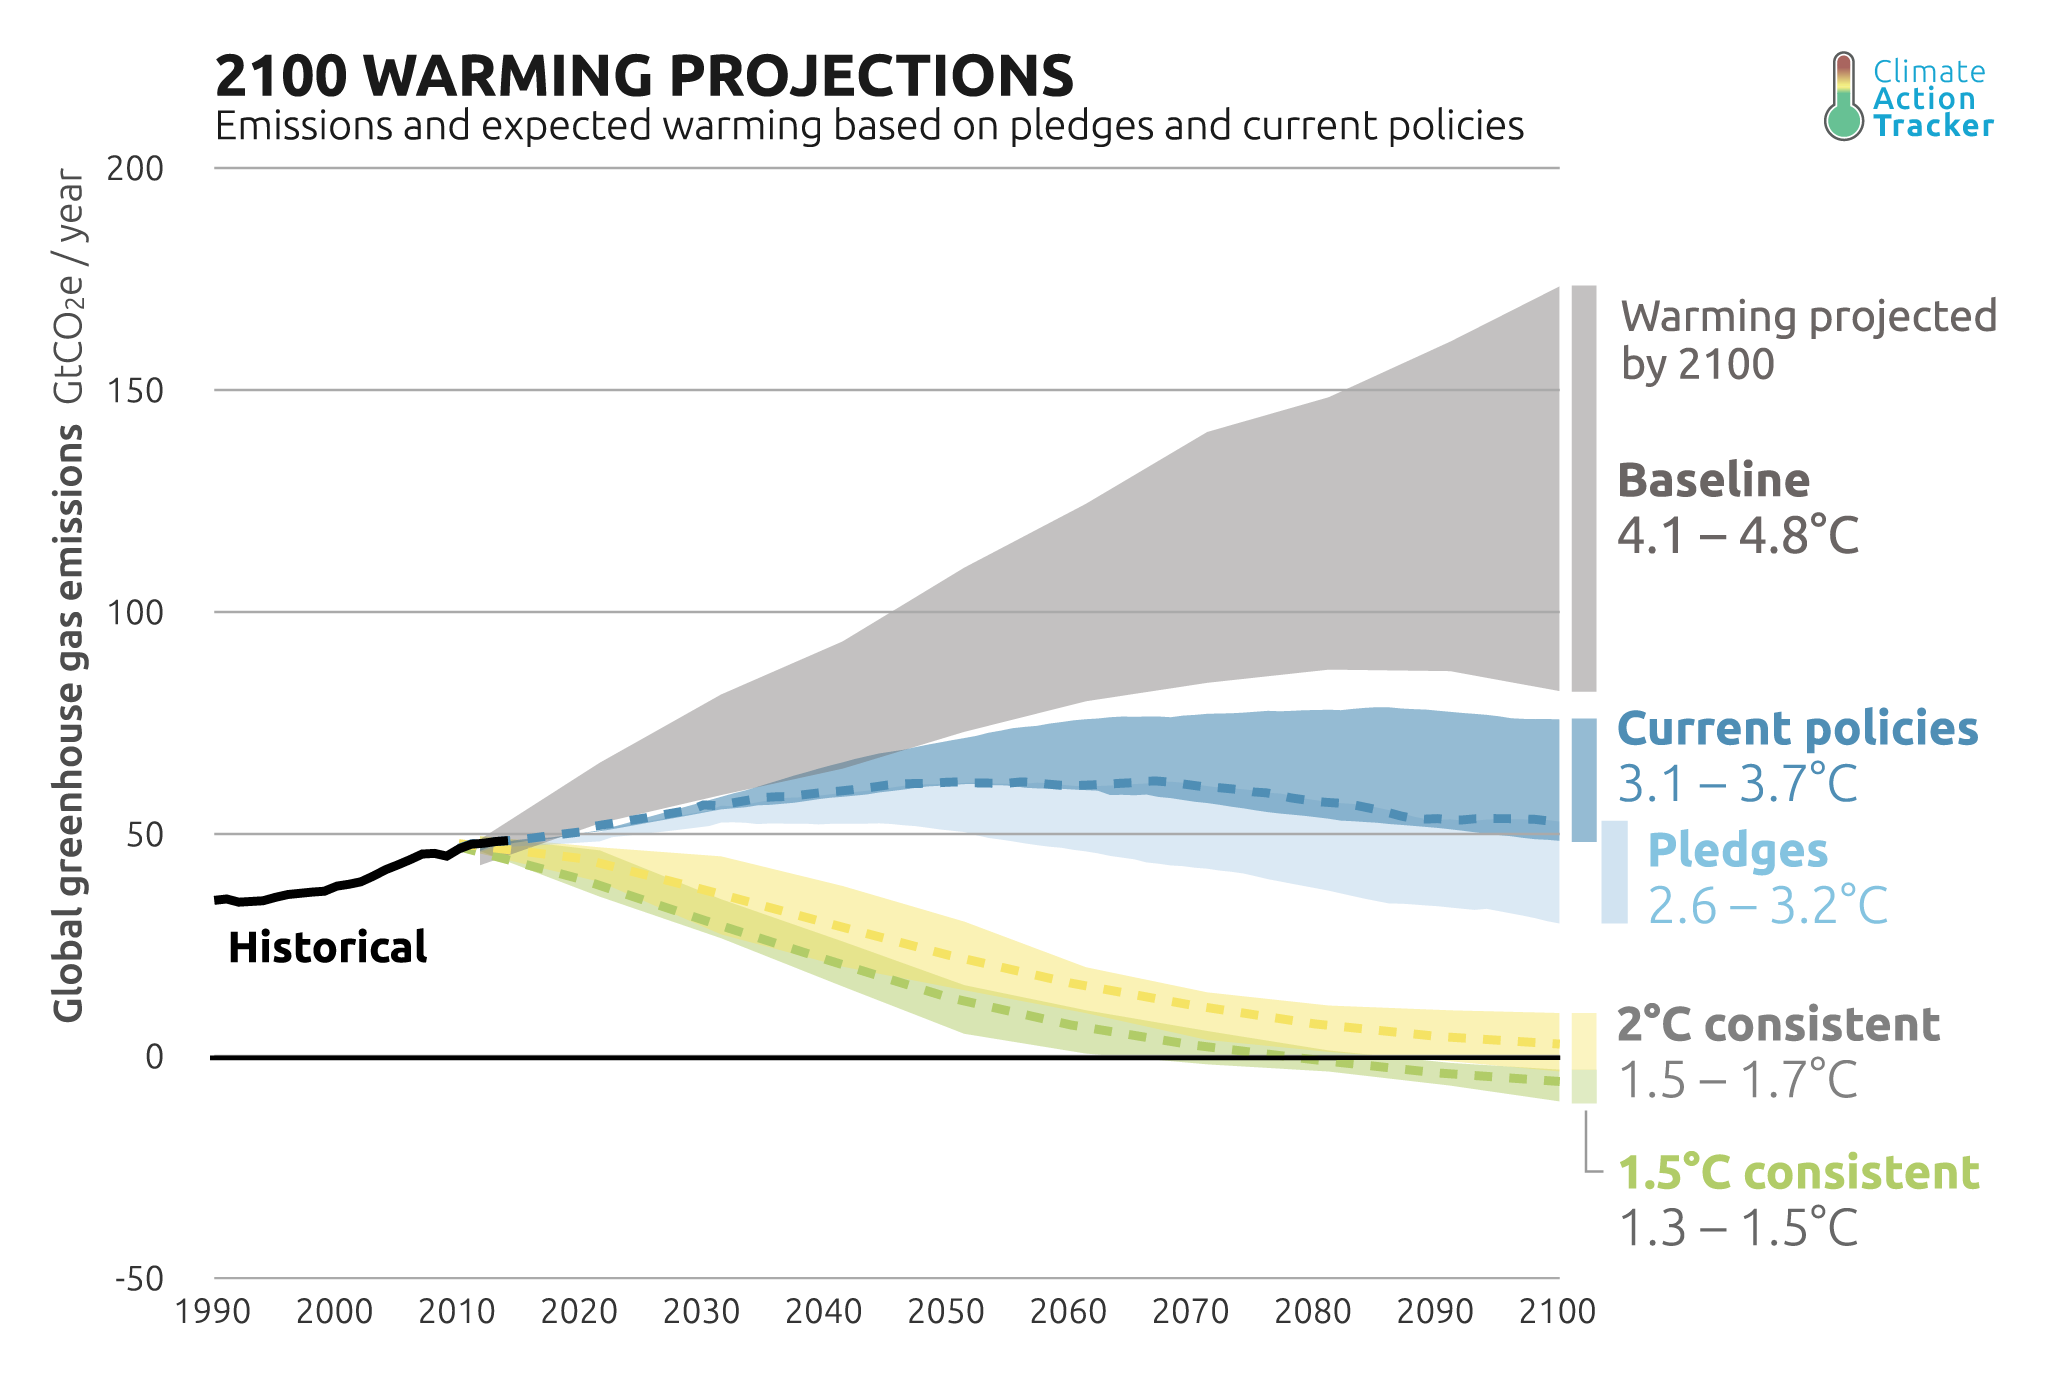
\includegraphics[width=\linewidth]{./Images/CAT-2100WarmingProjections-2017_11.png}
\caption{\label{fig:CountriesCommitment} \href{https://climateactiontracker.org/media/images/CAT-2100WarmingProjections-2017.11.original.png}{\tiny Source: Climate Action Tracker }}
\end{figure}
\end{frame}


\begin{frame}[allowframebreaks]
\frametitle{Reference}
\tiny
\bibliographystyle{apalike}
\bibliography{/media/work/Literature/Antarctica/litt_report/litt.bib}
\end{frame}

\end{document}


